\section{Simultaneous fits at $P_L=-1,-3,-4$}
\label{app:fit_results}

\begin{table*}[!t]
\caption{Parameters and global correlated $\chi^2/\text{dof}$ of the simultaneous fits at $P_L=-1,-3,-4$ ($|\vect b|\ge3a$, $6\le\eta\le10$, common $f$). The parameters of $\tAmp_{2B}^{\text{Re}}$ are $a,c,d,k_1,k_2,j$, those of $\tAmp_{2B}^{\text{Im}}$ are $a'',c'',d'',j''$ and those of $\tAmp_{12B}^{\text{Re}}$ are $a',c',d',j'$ in Eqs.~\eqref{eq:model_ReA2B}--\eqref{eq:model_ReA12B}. The fit at $P_L=-2$ is given in Table~\ref{tab:fit_params_P2}.}
\label{tab:fit_params}
\footnotesize
\setlength{\tabcolsep}{1.5pt}
\begin{ruledtabular}
\begin{tabular}{lccc}
 & $P_L=-1$ & $P_L=-3$ & $P_L=-4$ \\
\hline
$a$ & $3.863(11)$ & $4.0061(31)$ & $4.0086(15)$ \\
$c$ & $0.336(40)$ & $0.45(12)$ & $0.27(21)$ \\
$d$ & $0.1630(74)$ & $0.136(11)$ & $0.122(13)$ \\
$k_1$ & $12.288(23)$ & $12.284(11)$ & $12.2751(58)$ \\
$k_2$ & $-36.1965(45)$ & $-36.1973(19)$ & $-36.19925(89)$ \\
$j$ & $1.627(25)$ & $2.085(10)$ & $2.0654(56)$ \\
\hline
$a''$ & $0.267(13)$ & $0.328(11)$ & $0.269(13)$ \\
$c''$ & $0.2253(69)$ & $0.163(15)$ & $0.264(47)$ \\
$d''$ & $0.2205(66)$ & $0.147(13)$ & $0.196(14)$ \\
$j''$ & $1.108(21)$ & $1.057(15)$ & $1.0084(79)$ \\
\hline
$a'$ & $0.658(22)$ & $0.569(13)$ & $0.5824(55)$ \\
$c'$ & $0.0773(46)$ & $0.100(17)$ & $0.116(19)$ \\
$d'$ & $0.0747(43)$ & $0.094(16)$ & $0.102(18)$ \\
$j'$ & $2.0054(90)$ & $1.9969(49)$ & $2.0059(34)$ \\
\hline
$f$ & $0.4702(46)$ & $0.540(15)$ & $0.577(19)$ \\
\hline
$\chi^2/\text{dof}$ & $1.85(10)$ & $0.712(66)$ & $0.434(51)$ \\
\end{tabular}
\end{ruledtabular}
\end{table*}

\begin{table*}
\caption{Key parameters of the separable ansätze and the coupled power law at $P_L=-1$, $-3$ and $-4$ (the $P_L=-2$ values are in Table~\ref{tab:separable}). The Gaussian-longitudinal fits at $P_L=-3$ and $-4$ return $c_{\text{im}}$ and $a_{\text{im}}$ within $0.002$ of the centres of their priors ($0.30$ and $0.26$) with very small errors, so these two parameters are not determined by the data in those fits.}
\label{tab:separable_params_app}
\scriptsize
\setlength{\tabcolsep}{2pt}
\begin{ruledtabular}
\begin{tabular}{lccc}
Ansatz at $P_L=-1$ & $c_{\text{im}}$ & $c_{\text{reA12B}}$ & $a_{\text{im}}$ \\
\hline
ExpPb\_Expb & $0.001(26)$ & $0.045(23)$ & $-0.167(16)$ \\
ExpPb\_PowerLawb & $0.004(25)$ & $0.028(24)$ & $-0.167(31)$ \\
GaussianPb\_Expb & $0.57(17)$ & $0.0038(69)$ & $+0.05(12)$ \\
GaussianPb\_PowerLawb & $0.602(48)$ & $0.0016(61)$ & $+0.168(92)$ \\
Coupled power law & $0.2253(69)$ & $0.0773(46)$ & $+0.267(13)$ \\
\hline
Ansatz at $P_L=-3$ & $c_{\text{im}}$ & $c_{\text{reA12B}}$ & $a_{\text{im}}$ \\
\hline
ExpPb\_Expb & $0.015(19)$ & $-0.003(17)$ & $-0.178(33)$ \\
ExpPb\_PowerLawb & $0.021(17)$ & $-0.020(19)$ & $-0.197(30)$ \\
GaussianPb\_Expb & $0.3016(15)$ & $0.0016(15)$ & $+0.25982(16)$ \\
GaussianPb\_PowerLawb & $0.30081(78)$ & $0.0007(15)$ & $+0.259914(83)$ \\
Coupled power law & $0.163(15)$ & $0.100(17)$ & $+0.328(11)$ \\
\hline
Ansatz at $P_L=-4$ & $c_{\text{im}}$ & $c_{\text{reA12B}}$ & $a_{\text{im}}$ \\
\hline
ExpPb\_Expb & $0.458(16)$ & $0.033(33)$ & $+0.186(43)$ \\
ExpPb\_PowerLawb & $0.422(18)$ & $0.005(38)$ & $+0.212(27)$ \\
GaussianPb\_Expb & $0.29999997(28)$ & $0.0043(27)$ & $+0.260000002(17)$ \\
GaussianPb\_PowerLawb & $0.29999999(12)$ & $0.0025(33)$ & $+0.2600000007(74)$ \\
Coupled power law & $0.264(47)$ & $0.116(19)$ & $+0.269(13)$ \\
\end{tabular}
\end{ruledtabular}
\end{table*}


\begin{figure*}[!tp]
\centering
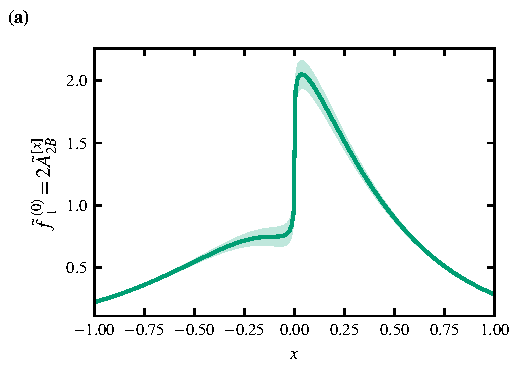
\includegraphics[width=\panelw]{figures/panels/xdep/xdep4_PL1_f1.pdf}\hfill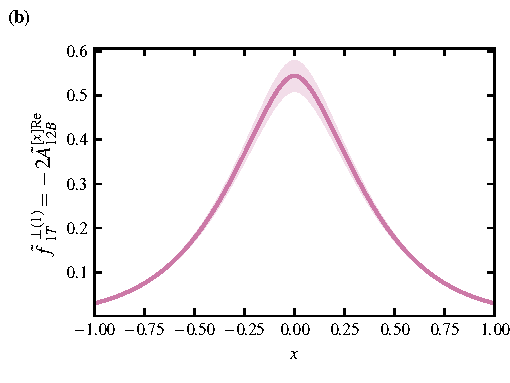
\includegraphics[width=\panelw]{figures/panels/xdep/xdep4_PL1_f1T.pdf}\par
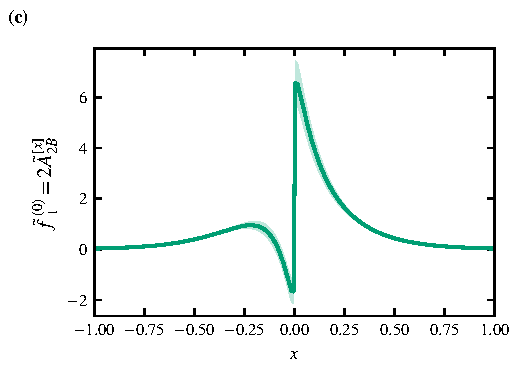
\includegraphics[width=\panelw]{figures/panels/xdep/xdep4_PL3_f1.pdf}\hfill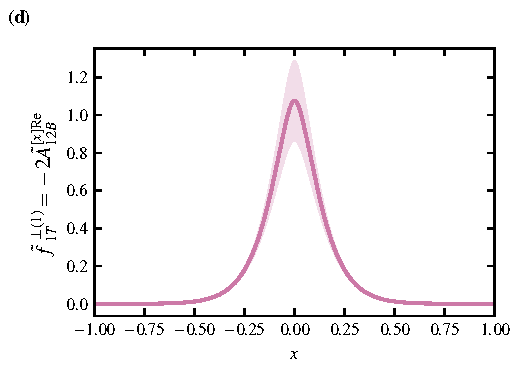
\includegraphics[width=\panelw]{figures/panels/xdep/xdep4_PL3_f1T.pdf}\par
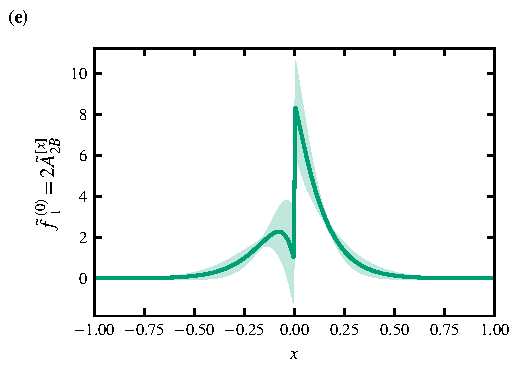
\includegraphics[width=\panelw]{figures/panels/xdep/xdep4_PL4_f1.pdf}\hfill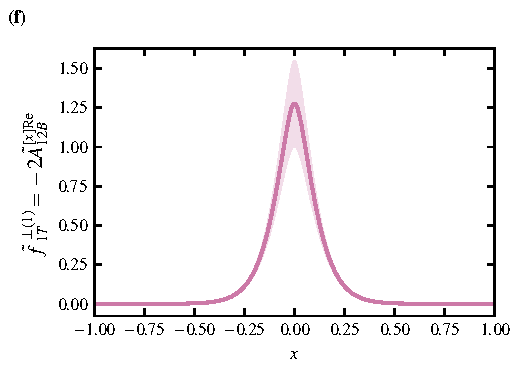
\includegraphics[width=\panelw]{figures/panels/xdep/xdep4_PL4_f1T.pdf}
\caption{$x$ dependence at $b^2=9a^2$ of $\tilde f_1^{(0)}$ (left) and $\tilde f_{1T}^{\perp(1)}$ (right) at $P_L=-1$ ($\hat\zeta=0.090772$, panels a, b), $-3$ ($0.539684$, c, d) and $-4$ ($0.785756$, e, f). Bands are Jackknife uncertainties.}
\label{fig:ft_xdep_P1}
\end{figure*}

\begin{figure*}[!tp]
\centering
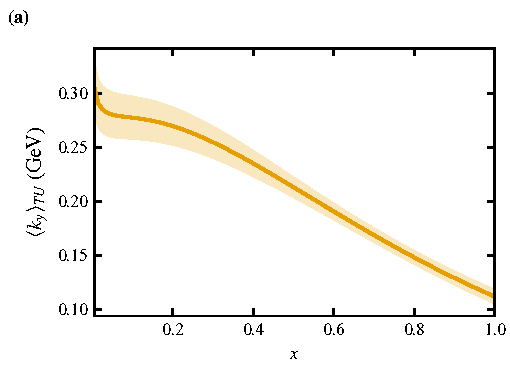
\includegraphics[width=\panelw]{figures/panels/xdep/xdep4_PL1_ky.pdf}\hfill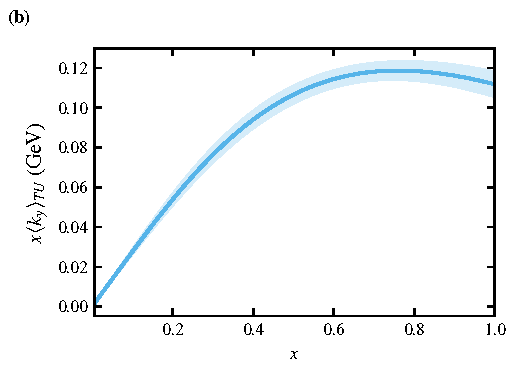
\includegraphics[width=\panelw]{figures/panels/xdep/xdep4_PL1_xky.pdf}\par
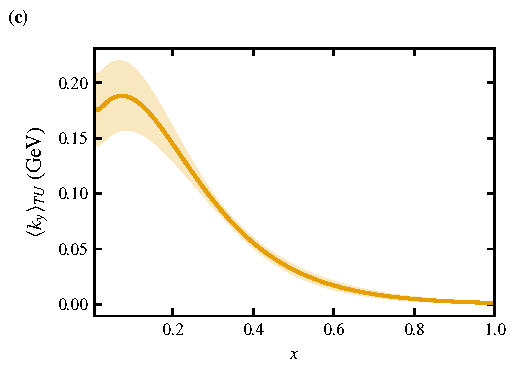
\includegraphics[width=\panelw]{figures/panels/xdep/xdep4_PL3_ky.pdf}\hfill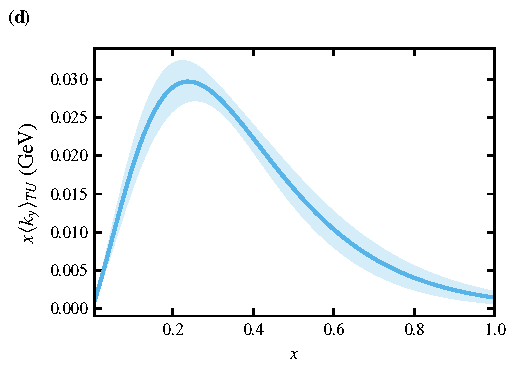
\includegraphics[width=\panelw]{figures/panels/xdep/xdep4_PL3_xky.pdf}\par
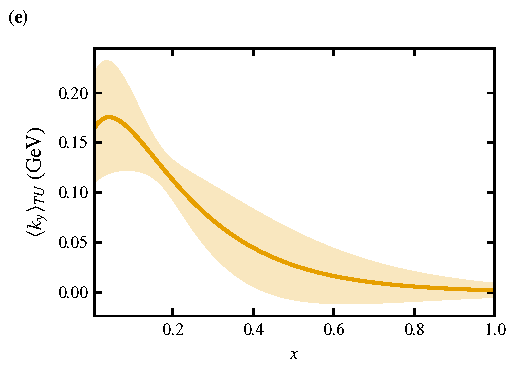
\includegraphics[width=\panelw]{figures/panels/xdep/xdep4_PL4_ky.pdf}\hfill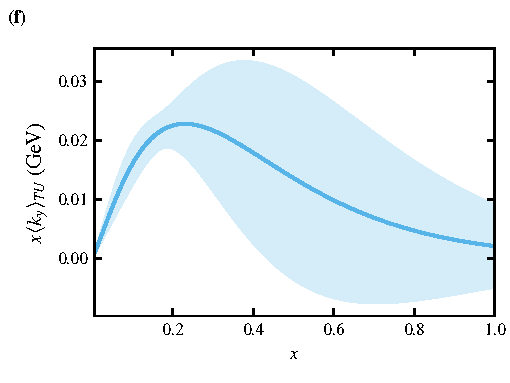
\includegraphics[width=\panelw]{figures/panels/xdep/xdep4_PL4_xky.pdf}
\caption{$x$ dependence at $b^2=9a^2$ of $\langle k_y\rangle_{TU}$ (left) and $x\langle k_y\rangle_{TU}$ (right) at $P_L=-1$ ($\hat\zeta=0.090772$, panels a, b), $-3$ ($0.539684$, c, d) and $-4$ ($0.785756$, e, f). Bands are Jackknife uncertainties.}
\label{fig:ft_xdep_P1_siv}
\end{figure*}
